% Fig 2 - Reconstructive (AE / Fukami) vs Predictive (JEPA).
%
% Restyled to the JFM block-diagram format (Sanchis-Agudo et al. style):
% soft pastel rounded containers, module NAMES as rotated labels OUTSIDE the
% colour boxes (the box holds the operation/architecture), pale tensor-shape
% boxes, dashed loss boxes, larger fonts.
%
% LEFT container  : reconstructive autoencoder, single column, L_AE pixel loss.
% RIGHT container : predictive JEPA, two columns (main + faint shared-weight
%                   target), L_JEPA latent loss, no decoder during training.
%
% Standalone-compilable: pdflatex fig2_predictive_vs_reconstructive.tex

\documentclass[border=12pt,tikz]{standalone}
\usepackage{tikz}
\usepackage{amsmath,amssymb}
\usetikzlibrary{positioning,arrows.meta,fit,shapes.geometric,calc,backgrounds}

\begin{document}

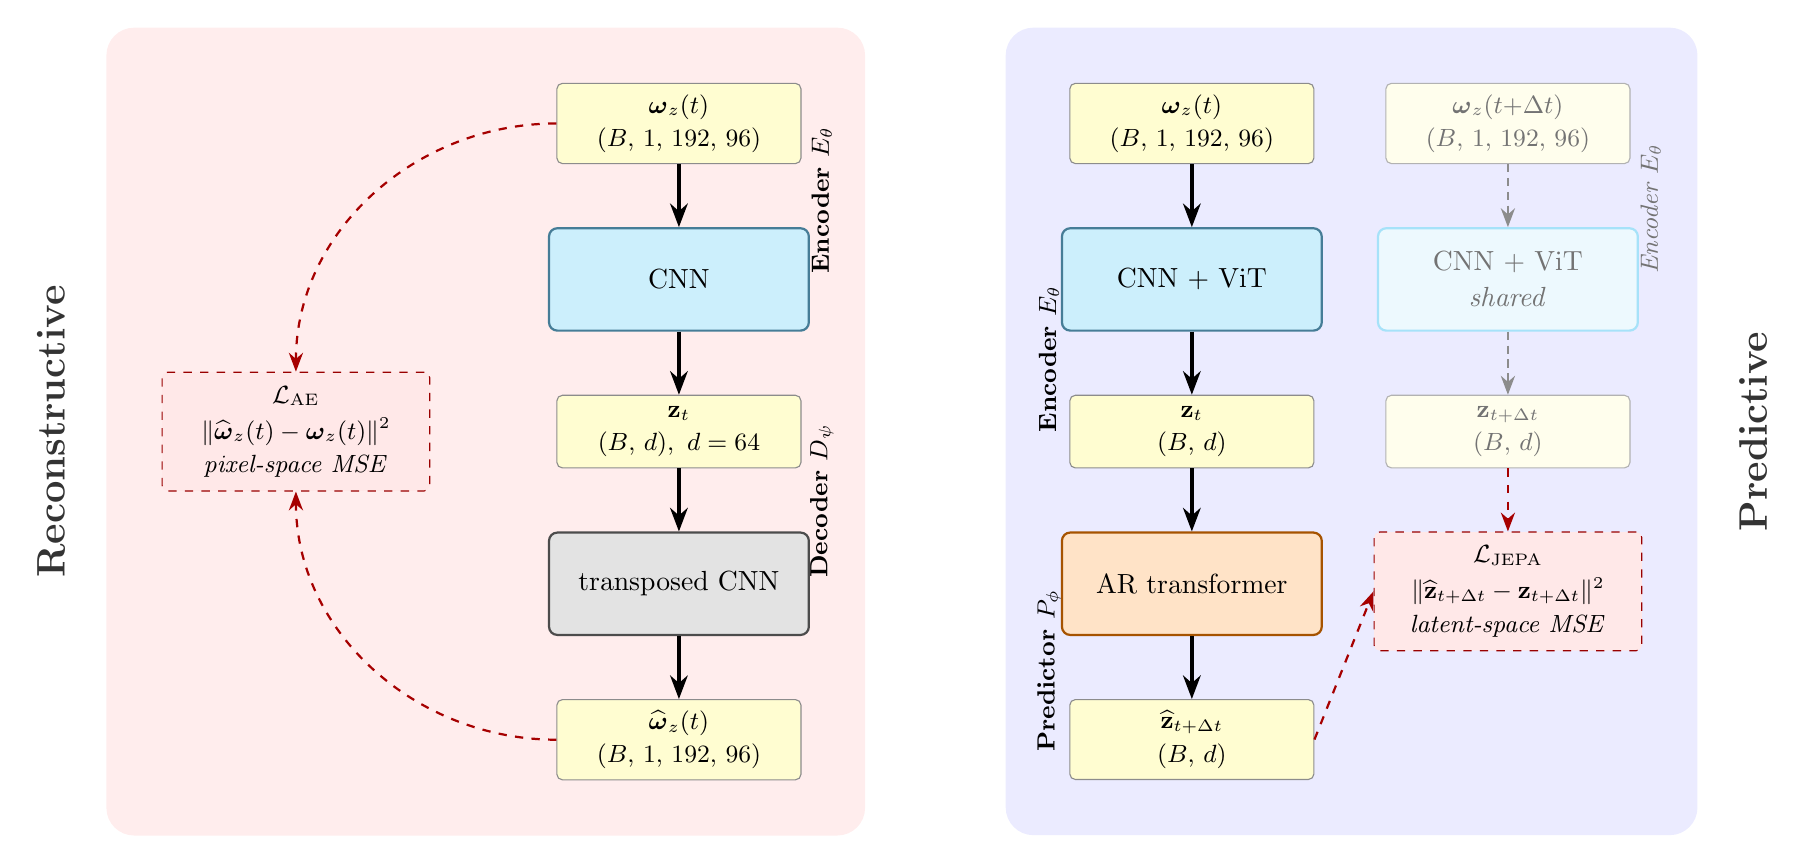
\begin{tikzpicture}[
    font=\normalsize,
    node distance=8mm,
    % operation blocks (colour-coded by role; the NAME sits outside, beside it)
    op/.style={draw, rounded corners=3pt, align=center, inner sep=6pt, thick,
               minimum width=33mm, minimum height=13mm},
    encoder/.style={op, fill=cyan!20,  draw=cyan!55!black},
    decoder/.style={op, fill=gray!22,  draw=gray!60!black},
    predictor/.style={op, fill=orange!22, draw=orange!65!black},
    encfaint/.style={op, fill=cyan!7, draw=cyan!35, text=black!55},
    % tensor-shape annotation boxes
    tbox/.style={draw=black!45, rounded corners=2pt, fill=yellow!18,
                 align=center, inner sep=4pt, font=\small,
                 minimum width=31mm, minimum height=9mm},
    tboxfaint/.style={tbox, fill=yellow!7, draw=black!30, text=black!55},
    % dashed loss boxes
    loss/.style={draw, rounded corners=2pt, dashed, fill=red!9, draw=red!60!black,
                 align=center, inner sep=5pt, font=\small,
                 minimum width=34mm, minimum height=15mm},
    % module names: rotated, OUTSIDE the colour box
    mname/.style={rotate=90, font=\small\bfseries, align=center, inner sep=2pt},
    mnamefaint/.style={mname, text=black!55, font=\small\itshape},
    arr/.style={-{Stealth[length=3mm]}, very thick},
    arrf/.style={-{Stealth[length=2.4mm]}, thick, black!45, densely dashed},
    larr/.style={-{Stealth[length=2.4mm]}, dashed, thick, red!65!black},
    side/.style={font=\Large\bfseries, rotate=90, align=center, text=black!80}
  ]

  % ===================== LEFT: reconstructive autoencoder =====================
  \node[tbox] (aein) {$\boldsymbol{\omega}_z(t)$ \\[1pt] $(B,\,1,\,192,\,96)$};
  \node[encoder, below=of aein] (aeenc) {CNN};
  \node[tbox, below=of aeenc] (aez) {$\mathbf{z}_t$ \\[1pt] $(B,\,d),\ d=64$};
  \node[decoder, below=of aez] (aedec) {transposed CNN};
  \node[tbox, below=of aedec] (aeout) {$\widehat{\boldsymbol{\omega}}_z(t)$ \\[1pt] $(B,\,1,\,192,\,96)$};

  % module names outside (to the right of each colour box)
  \node[mname, right=1.5mm of aeenc] {Encoder $E_{\theta}$};
  \node[mname, right=1.5mm of aedec] {Decoder $D_{\psi}$};

  \draw[arr] (aein)  -- (aeenc);
  \draw[arr] (aeenc) -- (aez);
  \draw[arr] (aez)   -- (aedec);
  \draw[arr] (aedec) -- (aeout);

  \node[loss, left=16mm of aez] (aeloss)
    {$\mathcal{L}_{\mathrm{AE}}$ \\[2pt]
     $\|\widehat{\boldsymbol{\omega}}_z(t)-\boldsymbol{\omega}_z(t)\|^{2}$ \\[1pt]
     \emph{pixel-space MSE}};
  \draw[larr] (aein.west) to[out=180,in=90]  (aeloss.north);
  \draw[larr] (aeout.west) to[out=180,in=-90] (aeloss.south);

  % ===================== RIGHT: predictive JEPA =====================
  \node[tbox, right=34mm of aein] (jin) {$\boldsymbol{\omega}_z(t)$ \\[1pt] $(B,\,1,\,192,\,96)$};
  \node[tboxfaint, right=9mm of jin] (jintgt)
    {$\boldsymbol{\omega}_z(t{+}\Delta t)$ \\[1pt] $(B,\,1,\,192,\,96)$};

  \node[encoder, below=of jin] (jenc) {CNN $+$ ViT};
  \node[encfaint, below=of jintgt] (jenctgt) {CNN $+$ ViT \\[1pt] \emph{shared}};

  \node[tbox, below=of jenc] (jz) {$\mathbf{z}_t$ \\[1pt] $(B,\,d)$};
  \node[tboxfaint, below=of jenctgt] (jztgt) {$\mathbf{z}_{t+\Delta t}$ \\[1pt] $(B,\,d)$};

  \node[predictor, below=of jz] (jpred) {AR transformer};
  \node[tbox, below=of jpred] (jzhat) {$\widehat{\mathbf{z}}_{t+\Delta t}$ \\[1pt] $(B,\,d)$};

  % module names outside (to the left of each main-column colour box)
  \node[mname, left=1.5mm of jenc] {Encoder $E_{\theta}$};
  \node[mname, left=1.5mm of jpred] {Predictor $P_{\phi}$};
  \node[mnamefaint, right=1.5mm of jenctgt] {Encoder $E_{\theta}$};

  \draw[arr]  (jin)   -- (jenc);
  \draw[arr]  (jenc)  -- (jz);
  \draw[arr]  (jz)    -- (jpred);
  \draw[arr]  (jpred) -- (jzhat);
  \draw[arrf] (jintgt)  -- (jenctgt);
  \draw[arrf] (jenctgt) -- (jztgt);

  \node[loss, below=of jztgt] (jloss)
    {$\mathcal{L}_{\mathrm{JEPA}}$ \\[2pt]
     $\|\widehat{\mathbf{z}}_{t+\Delta t}-\mathbf{z}_{t+\Delta t}\|^{2}$ \\[1pt]
     \emph{latent-space MSE}};
  \draw[larr] (jztgt.south) -- (jloss.north);
  \draw[larr] (jzhat.east) -- (jloss.west);

  % ===================== pastel containers + side labels =====================
  \begin{scope}[on background layer]
    \node[fill=red!7, rounded corners=10pt, inner sep=7mm,
          fit=(aein)(aeenc)(aez)(aedec)(aeout)(aeloss)] (lframe) {};
    \node[fill=blue!8, rounded corners=10pt, inner sep=7mm,
          fit=(jin)(jintgt)(jenc)(jenctgt)(jz)(jztgt)(jpred)(jzhat)(jloss)] (rframe) {};
  \end{scope}

  % side labels: same vertical centre (image middle), aligned across both panels
  \coordinate (gc) at ($(lframe.center)!0.5!(rframe.center)$);
  \node[side] at ($(lframe.west |- gc) + (-7mm,0)$) {Reconstructive};
  \node[side] at ($(rframe.east |- gc) + (7mm,0)$) {Predictive};

\end{tikzpicture}

\end{document}
